\documentclass{article}
\usepackage[fontset=ubuntu]{ctex}
\usepackage{graphics}
\usepackage{float}
\usepackage{graphicx}
\usepackage{pythonhighlight}
\usepackage{caption}
\usepackage{float}
\usepackage{multirow}
\usepackage[colorlinks=true, allcolors=blue]{hyperref}

\title{基于模糊推理的房源区位分析与推荐}
\author{崔晨昊 19307130084}
\date{June 2022}

\begin{document}

\maketitle

\section{摘要}

随着中国经济飞跃式发展,城市化水平不断提高,国民对房源需求的个性化趋势也越来越明显。然而,房源所处的区位信息往往无法第一时间被相关群体掌握,客观上造成了一定的信息不对等。同时,庞杂的房源数据也使得个性化需求的匹配难以进行。本研究搭建了一个基于模糊推理的房源推荐专家系统,并使用上海市杨浦区3万多条数据进行实验。系统实现了对房源区位条件的综合分析,一定程度上解决了用户的个性化房源区位需求\footnote{代码开源于\href{https://github.com/Unparalleled-Calvin/AI-PJ}{https://github.com/Unparalleled-Calvin/AI-PJ}}。

\section{选题背景}

一般来说,消费者在面对诸多住房选择时,往往很难做出决定~\cite{bg}。在其心理预先有一定偏好的情况下,盲目选择的房源大多最终只是差强人意。这些偏好大多与价格、楼层、升值空间、自然环境、交通设施、教育资源、消费场所、娱乐设施等因素有关。例如,有孩子教育需求的家长往往更倾向于选择学区内房源,而年轻群体则更愿意将住所放在消费场所丰富的商圈附近。

当前房源推荐平台软件等大多着眼于价格、房型等房源的内部属性,对目标处房源进行简单的筛选和显示,而对房源区位属性的考量却仅囊括交通因素。对于用户更加丰富的个性化需求,多数平台需要转交人工服务进行处理。另外,用户消费的需求也不尽相同。以不动产置业、居住等为需求的群体更多关注商品商品房源,而以旅行、出差等为需求的群体,则更多关注宾馆、民宿、公寓等短租房源,平台对于这几种需求的处理也较为粗放。

\begin{figure}[htbp]
\centering
    \begin{tabular}{cc}
        \begin{minipage}[t]{2in}
        \centering
        
\includegraphics[height=0.4\textheight]{./pic/贝壳找房.jpg}
        \caption{贝壳找房房源筛选示例}
        \label{贝壳找房}
        \end{minipage}
    %%   
        \begin{minipage}[t]{2in}
        \centering
        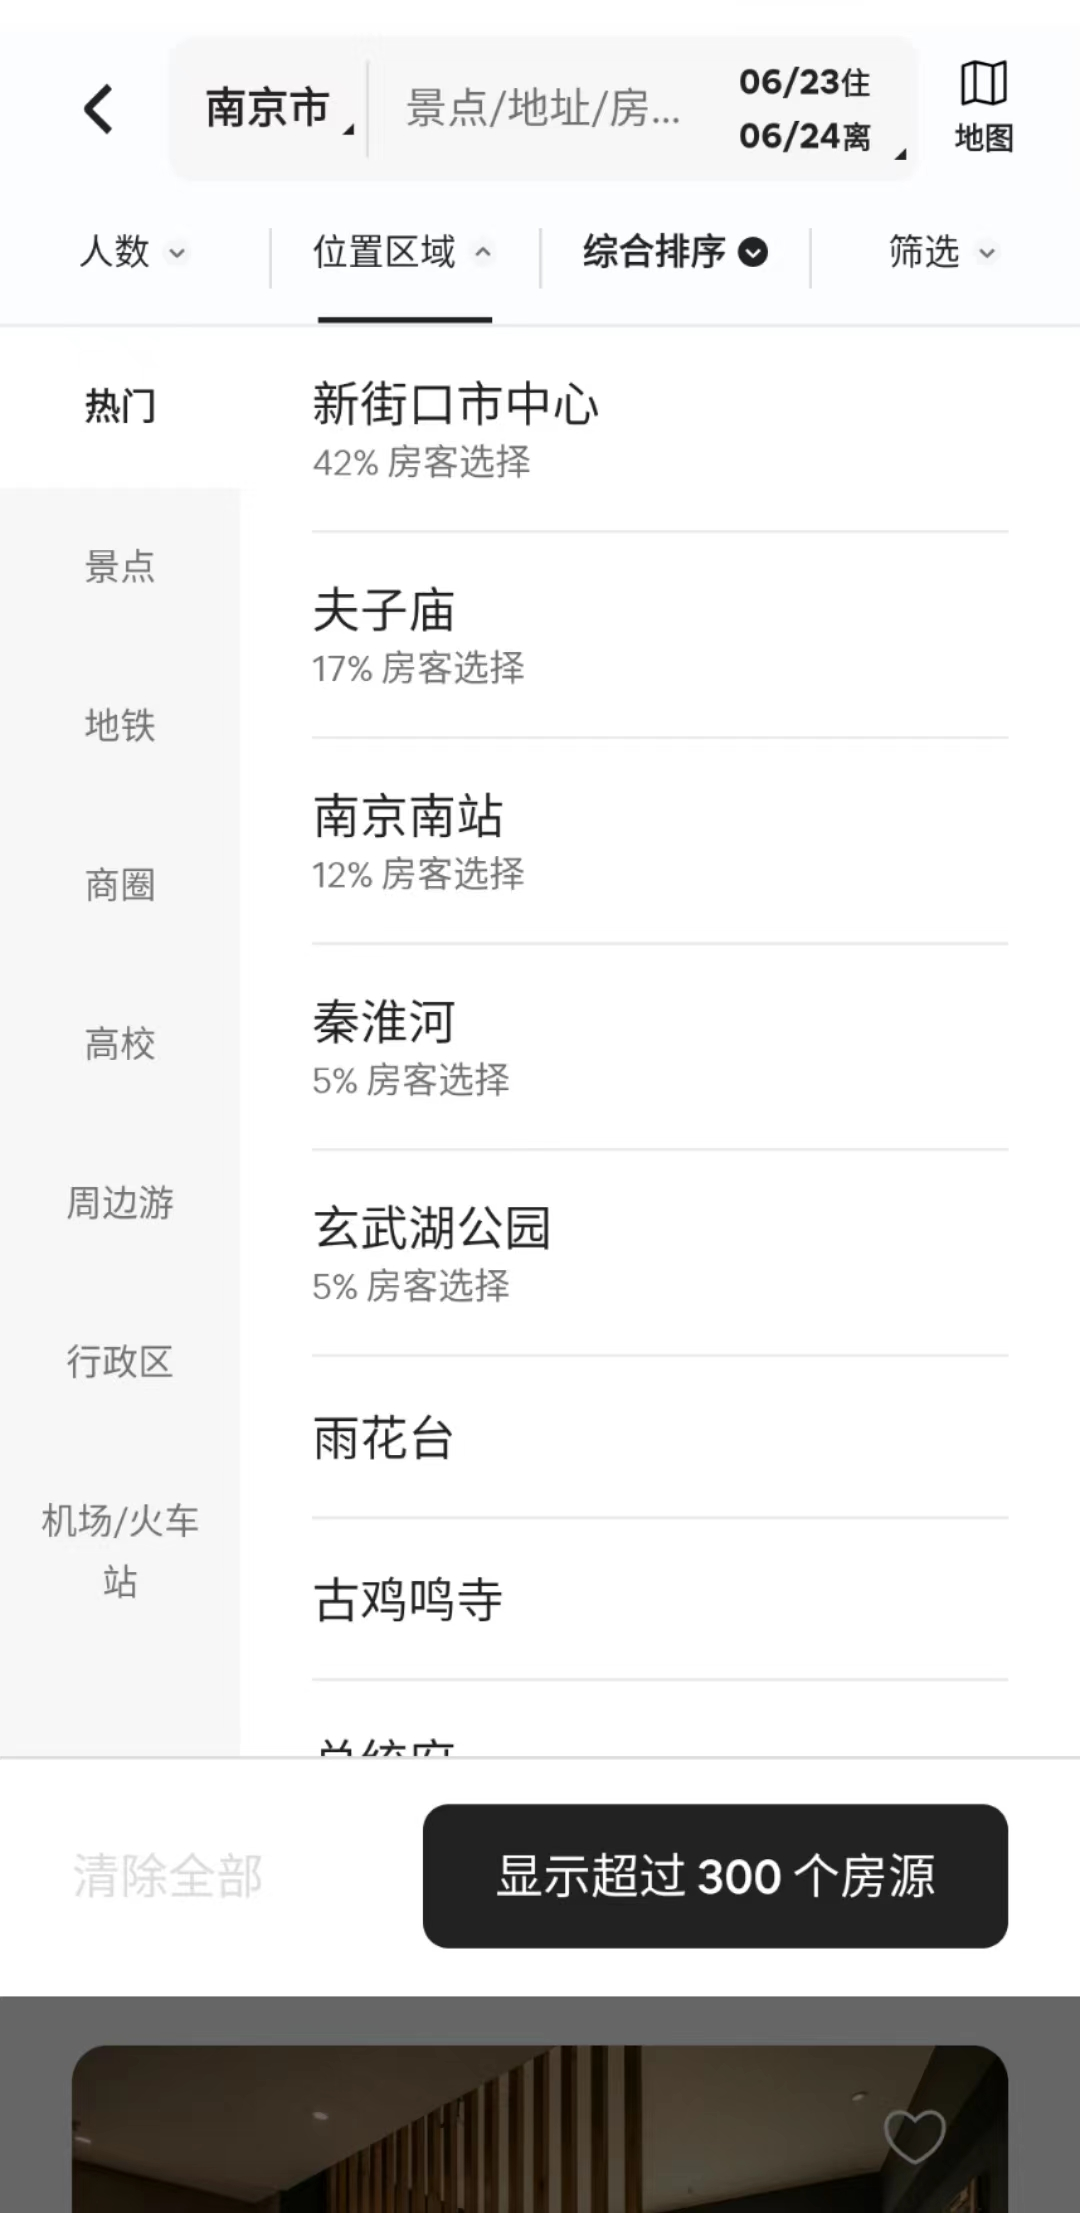
\includegraphics[height=0.4\textheight]{./pic/爱彼迎.jpg}
        \caption{爱彼迎房源筛选示例}
        \label{爱彼迎}
        \end{minipage}
    \end{tabular}
\end{figure}

以贝壳找房和爱彼迎两家比较有代表性的软件为例,可以看到,目前两款软件均主要针对房源所处的行政区域、房源价格、户型等进行了筛选排序。如果要进一步了解房源信息,则需在线咨询房源经纪人,极大地增加了沟通成本。同时,贝壳找房主打商品房和长租房,对于房源周边环境的分析较少,难以满足旅游群体的需求(图\ref{贝壳找房})。而爱彼迎主打旅游民宿短租,对民宿周边景点环境等分析较多,但难以满足商品房购置群体的需求(图\ref{爱彼迎})。

因此,为了满足各类人群的房源个性化区位需求,有必要开发一款能够综合地理信息数据并进行房源区位条件综合分析的专家系统,帮助相关人群找到称心如意的房源。

\section{前置知识}
\subsection{房源区位需求分析}

首先,本研究需要明确相关人群的对房源区位条件的具体需求。研究~\cite{需求分析}通过对上海市房源溢价进行分析,在临近设施方面得到了如下结论:

\begin{itemize}
    \item 教育设施方面,\textbf{公立重点初中}、\textbf{小学}周边溢价效应明显,与公立基础教育资源“就近入学”的学区安排有紧密关系。虽然高中没有明确的学区安排,但\textbf{示范性高中}周边住房价格也具有溢价效应。重点大学周边住房价格和租金没有溢价效应,说明高等教育资源的临近性不是住房选择的主要考虑因素。
    
    \item 医疗设施方面,代表优质医疗资源的三级\textbf{综合型医院}对周边住房价格和租金产生了一定程度的影响。
    
    \item 休闲生活设施方面,\textbf{免费公园}周边社区的住房租金水平显著高于远离公园的社区,同时周边\textbf{餐馆}密度也对租金产生一定影响。
    
    \item 公共交通设施方面,\textbf{轨道交通}为租购群体的日常出行提供了便利,对站点周边住房价格和租金都有显著影响。
\end{itemize}

另外一方面,研究~\cite{poi分类}在计算社区综合吸引力时,也将生活设施分为交通、商业、文体、健康四个方面来考虑(图\ref{设施分类})。

\begin{figure}[htbp]
\centering
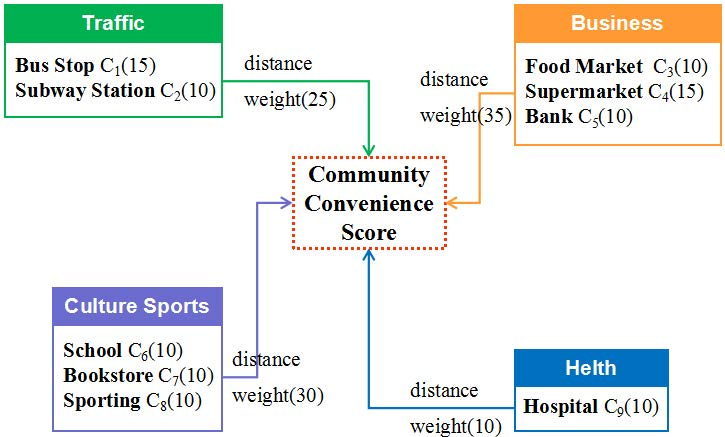
\includegraphics[width=0.9\textwidth]{./pic/设施分类.jpg}
\caption{研究~\cite{poi分类}使用的设施分类}
\label{设施分类}
\end{figure}

因此,本研究主要考虑教育设施、医疗设施、休闲设施、文旅设施、公共交通等因素,以房源周边设施丰富度来衡量该类设施对房源区位优势的贡献。而将用户的需求归纳为\textbf{教育}、\textbf{消费}、\textbf{医疗}、\textbf{旅游}、\textbf{交通}五个方面。

\subsection{区位优势量化}

区位优势的考量需要综合设施到房源的距离以及设施数量的影响。一般来说,距离越近,数量越多,区位优势更加明显。为了更好地量化评估设施对房源的影响,本研究使用Walk Score~\cite{walk}计算某处设施对于单个房源的增益。在Walk Score给出的曲线中(图\ref{walk score}),距离为0.25英里以内(步行时间5分钟),得分在100分左右;距离为1英里左右(步行时间20分钟),得分将衰减到15分;而距离为1.5英里左右(步行时间30分钟)时,得分将衰减到0分。

\begin{figure}[htbp]
\centering
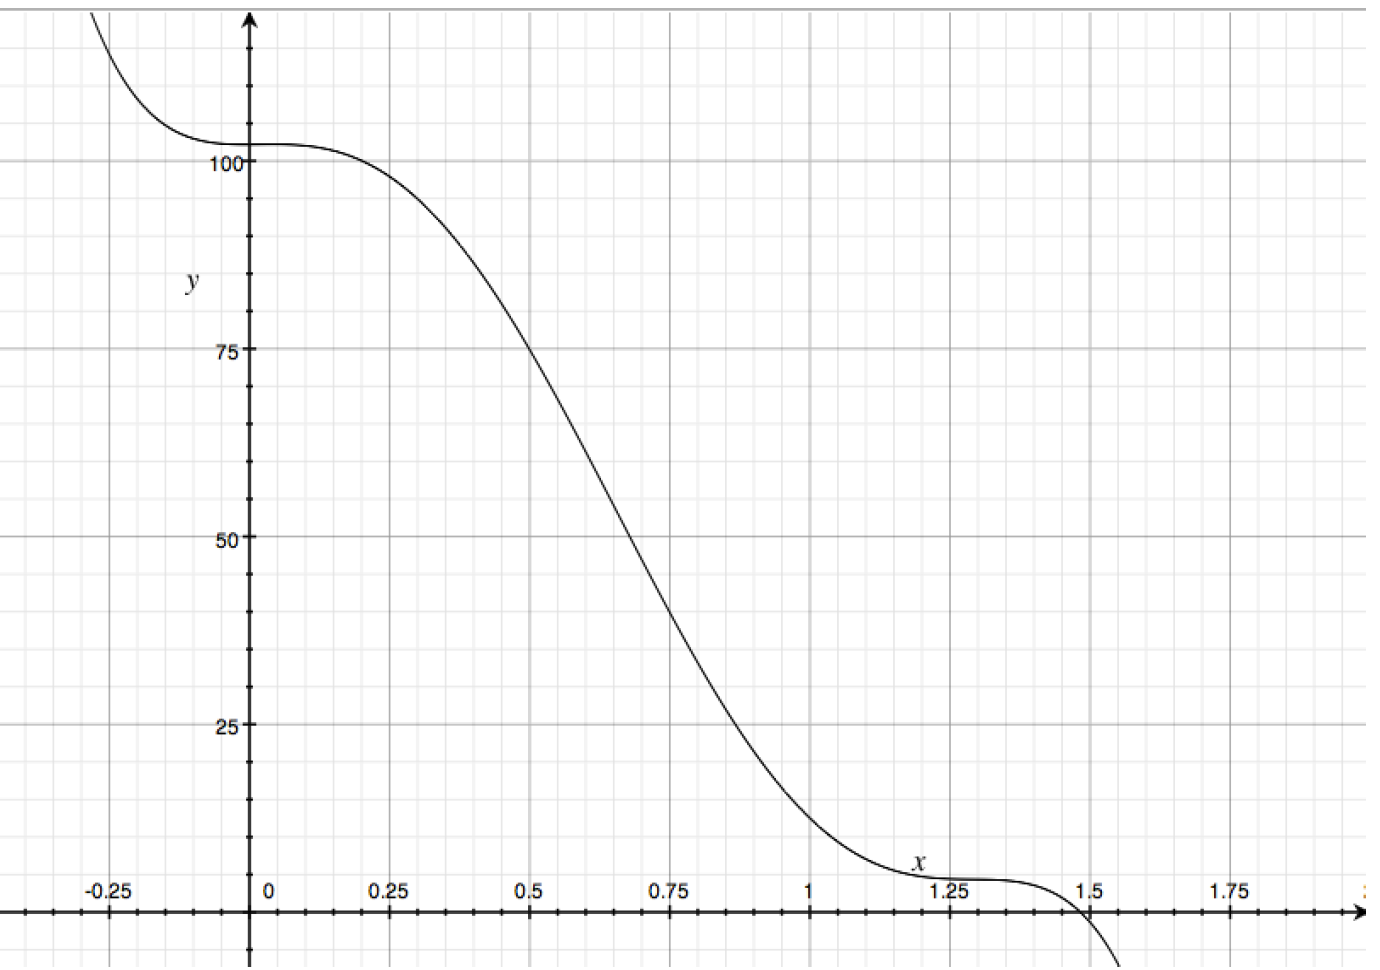
\includegraphics[width=0.9\textwidth]{./pic/walk score.png}
\caption{Walk Score}
\label{walk score}
\end{figure}

计算每个房源周边设施带来的区位优势,并将同种设施的得分予以\textbf{加和},即可得到该房源不同种类的得分。所有房源计算完毕后,可对同一项得分做\textbf{归一化处理},从而相对得到比较合理的区位优势量化结果。

\section{数据处理与模糊推理}

本研究使用了来自于上海杨浦区的37495条POI(Point of Interest)信息,每条记录包括该地点名称、所属的大类、中类、经纬度等信息(图\ref{数据示例})。经过初步统计,数据共含有旅游景点,交通设施,生活服务,运动健身,科教文化,休闲娱乐,餐饮美食,购物消费,政府机构,汽车相关,商务住宅,公司企业,行政地标,酒店住宿,医疗保健,金融机构,自然地物等17个大类,公园,广场,景点等172个中类细分地点类别。注意到数据中的商务住宅、酒店住宿两个大类即为本系统所推荐的房源范围,而其余景点、交通等POI即作为本系统区位分析的原始数据。

\begin{figure}[htbp]
\centering
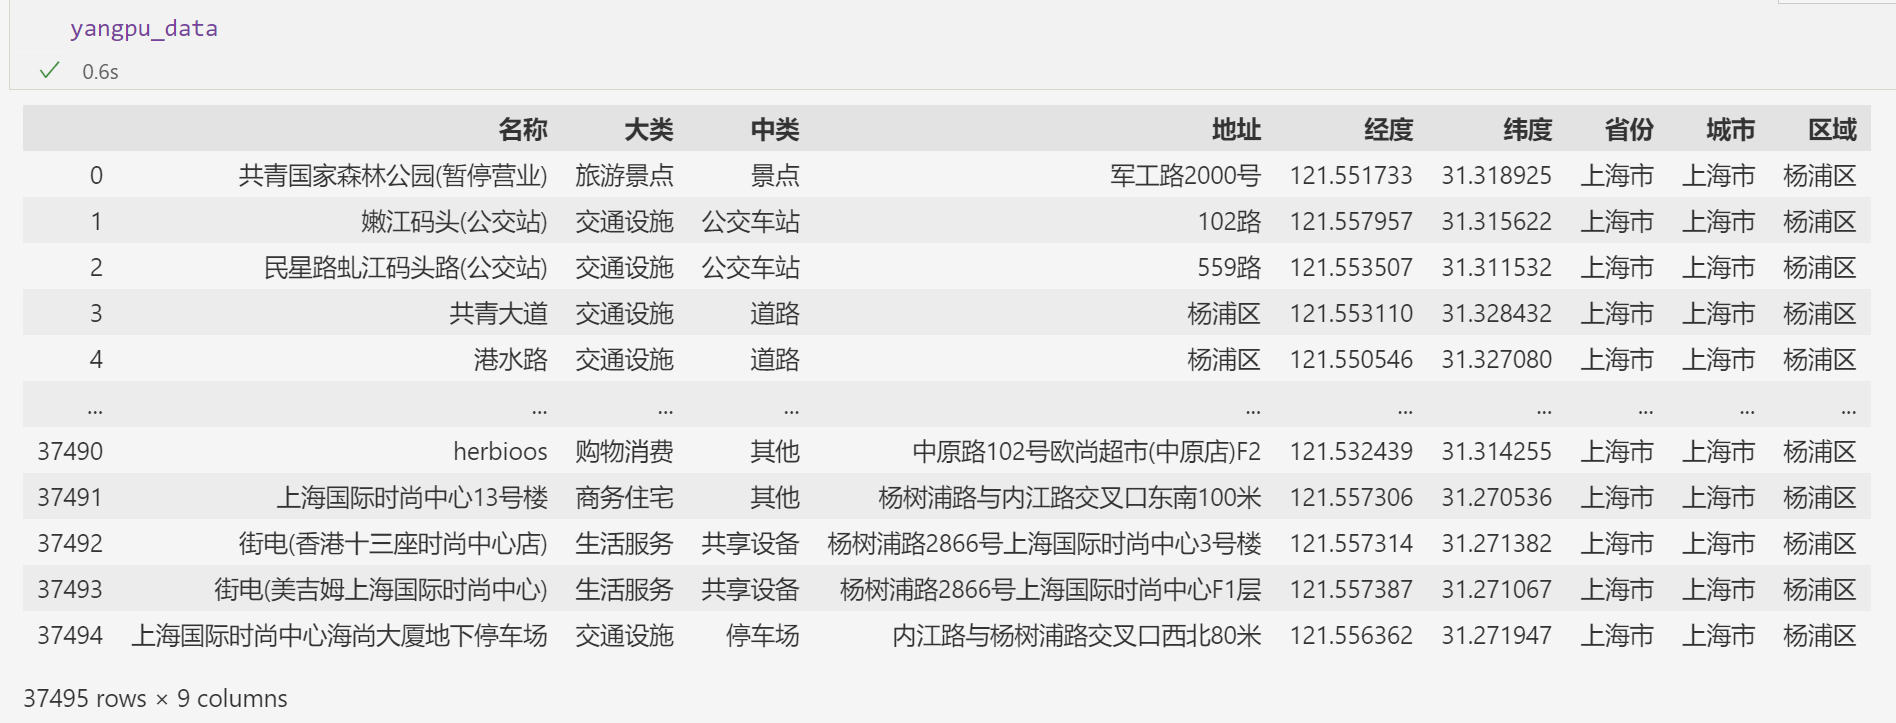
\includegraphics[width=0.9\textwidth]{./pic/数据示例.png}
\caption{杨浦区POI数据示例}
\label{数据示例}
\end{figure}

\begin{figure}[htbp]
\centering
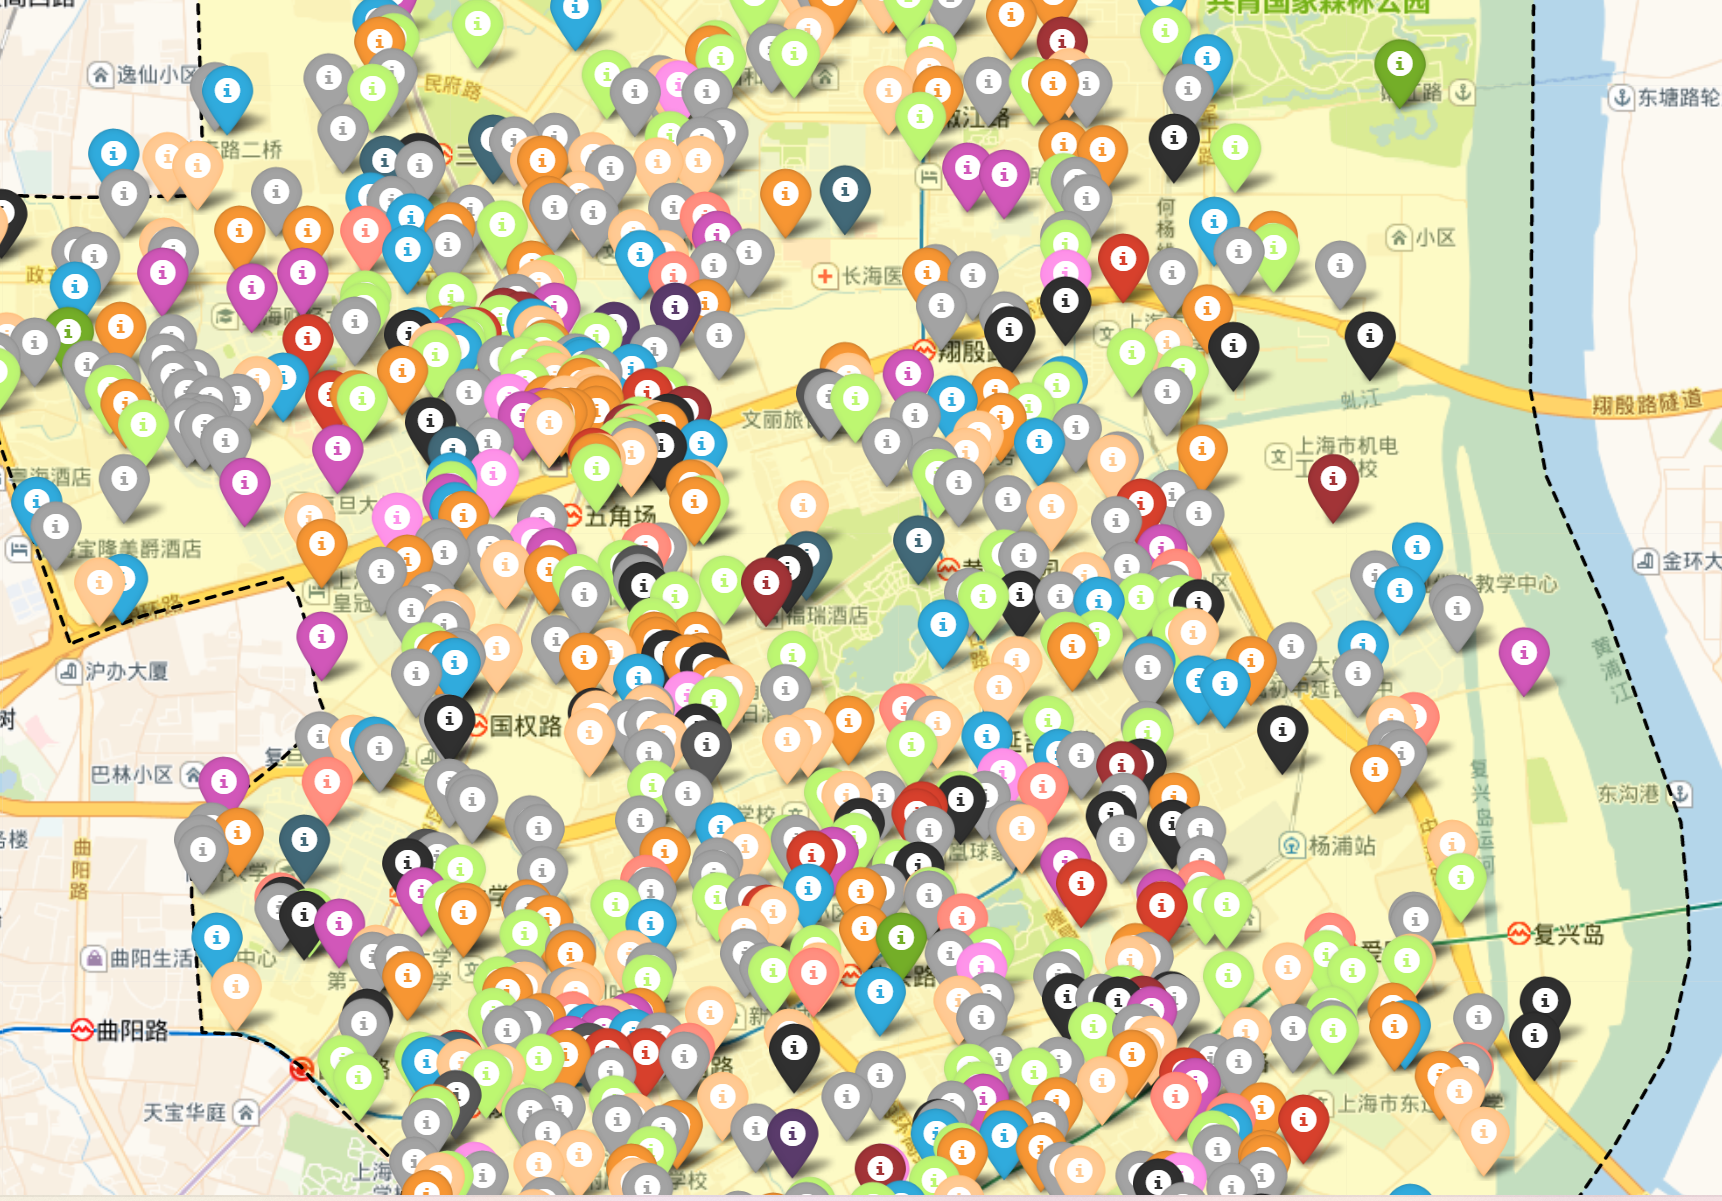
\includegraphics[width=0.9\textwidth]{./pic/地图示例.png}
\caption{POI分布可视化(已做抽样处理)}
\label{地图示例}
\end{figure}

为了更加直观地体现所使用的数据数据,利用Python的folium~\cite{folium}包进行地图绘制和点标注,做进一步的可视化处理。地图接口来自高德地图,同时使用了阿里云DataV.GeoAtlas工具得到杨浦区精确行政区域边界经纬度。选取1/10的商品房和1/50的其他类别POI在地图上标注(图\ref{地图示例})。

\begin{figure}[htbp]
\centering
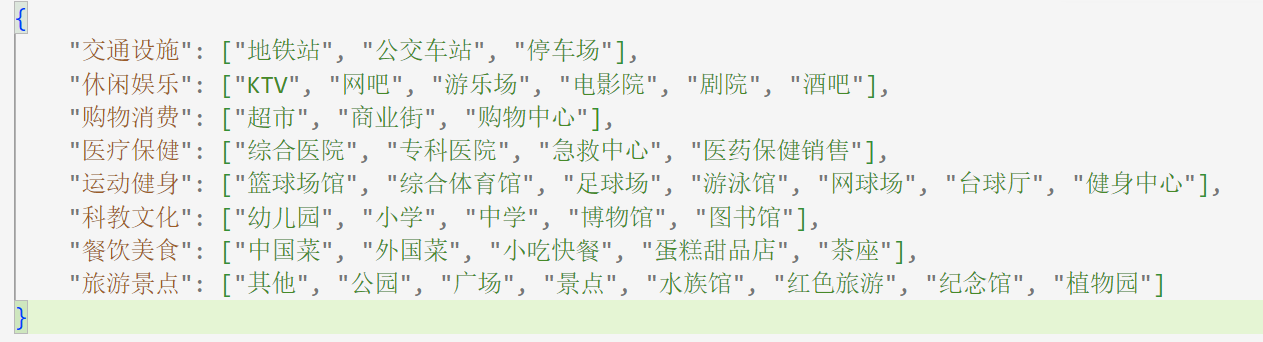
\includegraphics[width=0.9\textwidth]{./pic/输入设施.png}
\caption{输入设施类别}
\label{输入设施}
\end{figure}

根据房源区位需求分析,从数据集中筛选出8个大类40个中类,将大类设施得分作为输入变量(图\ref{输入设施}),同时以教育质量、消费场所、医疗健康、旅游资源、交通运输作为输出变量进行后续分析,符号表见表\ref{符号表}。

\begin{table}[htbp]
\centering
\begin{tabular}{|c|c|c|c|}
\hline
\multicolumn{2}{|c|}{输入变量表} & \multicolumn{2}{|c|}{输出变量表}\\ \hline
符号             & 含义             & 符号             & 含义\\ \hline
$transportation$ & 交通设施大类得分 & $Education$      & 教育质量 \\ \hline
$entertainment$  & 休闲娱乐大类得分 & $Comsuming$      & 消费场所 \\ \hline
$consuming$      & 购物消费大类得分 & $Health$         & 医疗健康 \\ \hline
$health$         & 医疗保健大类得分 & $Tourism$        & 旅游资源 \\ \hline
$sport$          & 运动健身大类得分 & $Transportation$ & 交通运输 \\ \hline 
$education$      & 科教文化大类得分 & \multicolumn{2}{|c|}{} \\ \hline
$restaurant$     & 餐饮美食大类得分 & \multicolumn{2}{|c|}{} \\ \hline 
$tourism$        & 旅游景点大类得分 & \multicolumn{2}{|c|}{} \\ \hline
\end{tabular}
\caption{符号表}
\label{符号表}
\end{table}

\subsection{Walk Score计算}
计算设施对于房源的影响需要有明确的函数表达式,然而研究~\cite{walk}并未给出Walk Score的函数公式。根据定义中的多个距离关键点以及图像趋势,可以使用scipy.interpolate包提供的interp1d函数对进行插值拟合,得出一个图形近似的函数对象用于计算。实验表明,使用四次函数进行拟合得到的效果最好。

\begin{python}
import numpy as np
from scipy import interpolate

# 插值拟合点
miles = [0, 0.125, 0.25, 0.5, 0.75, 1, 1.25, 1.5] #英里
scores = [100, 99.8, 97.5, 75, 40, 12.5, 5, 0] #分数

def mile2km(mile):
    factor = 0.62137119
    return mile/factor

kms = [mile2km(mile) for mile in miles]
func = interpolate.interp1d(kms, scores, kind="quadratic") #四次函数拟合
\end{python}

利用matplotlib画出函数图像(图\ref{拟合结果}),可以看出插值拟合得出的函数曲线和原文给出的Walk Score曲线基本相似。距离较近时得分基本不衰减,中距离时得分衰减效应明显,长距离下得分衰减至0。

\begin{figure}[htbp]
\centering
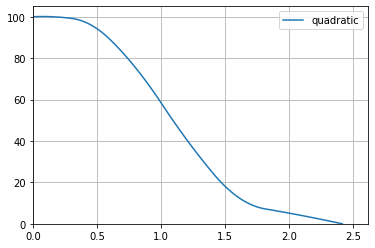
\includegraphics[width=0.9\textwidth]{./pic/拟合结果.png}
\caption{Walk Score拟合结果}
\label{拟合结果}
\end{figure}

\subsection{大类得分计算}

设施对房源的大类得分通过对大类下子类得分加和后归一化得出。归一化操作帮助统一不同评价的量化结果,其大小大体上可以区分不同房源在该类设施上的区位优势。当得分越大时,说明房源附近该类设施较多,自然有相关需求的人群会更加偏好这类房源。

\begin{python}
# 计算locations中的所有分数
def calc_one_type_scores(type, subtypes, data_dict, locations, norm = True): 
    scores = []
    for index, data in locations.iterrows():
        location = [data["纬度"], data["经度"]]
        #将大类下中类的得分做加和
        for subtype in subtypes:
            score += [calc_score(data_dict[subtype], location) 
        scores.append(score)
    #归一化处理
    if norm: 
        max_score, min_score = max(scores), min(scores)
        diff = max_score - min_score
        scores = [(score-min_score)/diff for score in scores]
    scores = pd.DataFrame(scores, columns=[type])
    return scores
\end{python}

\subsection{模糊推理}

\begin{table}[!ht]
\centering
\begin{tabular}{|c|c|c|c|c|c|}
\hline
\multicolumn{3}{|c|}{语言变量:大类得分$education$等} & \multicolumn{3}{|c|}{语言变量:教育质量$Education$} \\ \hline
语言值 & 符号 & 值范围 & 语言值 & 符号 & 值范围 \\ \hline
Good   & H    & [0.6, 1] & High   & H    & [0.8, 1] \\ \hline
Average& M    & [0.3, 0.7] & Medium & M    & [0.5, 0.85] \\ \hline
Poor   & L    & [0, 0.4] & Low    & L    & [0, 0.55] \\ \hline
\multicolumn{3}{|c|}{语言变量:消费场所$Consuming$} & \multicolumn{3}{|c|}{语言变量:医疗健康$Health$} \\ \hline
语言值 & 符号 & 值范围 & 语言值 & 符号 & 值范围 \\ \hline
Plenty & P    & [0.7, 1] & High   & H    & [0.8, 1] \\ \hline
Normal & N    & [0.3, 0.75] & Medium & M    & [0.5, 0.85] \\ \hline
Short  & S    & [0, 0.4] & Low    & L    & [0, 0.55] \\ \hline
\multicolumn{3}{|c|}{语言变量:旅游资源$Tourism$} & \multicolumn{3}{|c|}{语言变量:交通运输$Transportation$} \\ \hline
语言值 & 符号 & 值范围 & 语言值 & 符号 & 值范围 \\ \hline
Rich   & R    & [0.8, 1] & Convenient & C    & [0.7, 1] \\ \hline
Normal & N    & [0.5, 0.85] & Normal & N    & [0.4, 0.75] \\ \hline
Short  & S    & [0, 0.55] & Inconvenient  & I    & [0, 0.45] \\ \hline
\end{tabular}
\caption{语言变量及其范围}
\label{输出变量}
\end{table}

教育质量$Education$、消费场所$Consuming$、医疗健康$Health$、旅游资源$Tourism$、交通运输$Transportation$等五项输出语言变量由模糊推理给出结果。表\ref{输出变量}给出这些输出语言变量及其范围。需要注意的是,由于教育和医疗的质量对区位优势的影响更大,旅游资源整体上来说比较稀缺,这三者呈现出明显的头部效应,较积极的语言值范围总体占比较少。而交通和消费则相对分布比较均匀,因此较积极的语言值范围总体占比较大。

下面分别以教育质量,消费场所,医疗健康为例,构建模糊推理规则。在所有输入变量中,教育质量仅与科教文化大类得分有关(与之类似,交通运输只与交通设施有关)。因此,构建模糊推理规则如下:

\begin{python}
Rule: 1
IF education IS Good
THEN Education IS High
Rule: 2
IF education IS Average
THEN Education IS Medium
Rule: 3
IF education IS Poor
THEN Education IS Low
\end{python}


而消费场所与休闲娱乐大类、购物消费大类有关,且这二者对消费场所的影响是相同占比的(与之类似,旅游资源与旅游景点大类、购物消费大类有关)。因此,构建模糊推理规则如下:

\begin{python}
Rule: 4
IF entertainment IS Good 
OR consuming IS Good
THEN Consuming IS Plenty
Rule: 5
IF (entertainment IS Average AND consuming IS NOT Good) 
OR (consuming IS Average AND entertainment IS NOT Good)
THEN Consuming IS Normal
Rule: 6
IF entertainment IS Poor
AND consuming IS Poor
THEN Consuming IS Short
\end{python}

最后,医疗健康与医疗保健大类,运动健身大类有关。但前者应该在推理中占有更多的比重,当运动场所大类得分不佳时,应该以医疗保健大类得分作为主要参考。因此构建模糊推理规则如下:

\begin{python}
Rule: 7
IF health IS Good
OR sport IS Good
THEN Health IS High
Rule: 8
IF health IS Average
AND sport IS NOT Good
THEN Health IS Medium
Rule: 9
IF health IS Poor
AND sport IS NOT Good
THEN Health IS Low
\end{python}

使用python的skfuzzy~\cite{skfuzzy}包可以快速构建语言变量,配合numpy包进行模糊操作即可计算出最终结果。下面以医疗健康为例:

\begin{python}
import skfuzzy as fuzz
import numpy as np

score_range = np.arange(0, 1.1, 0.01)
#定义语言变量隶属函数
Good = fuzz.trimf(score_range, [0.6, 1, 1])
Average = fuzz.trimf(score_range, [0.3, 0.5, 0.7])
Poor = fuzz.trimf(score_range, [0, 0, 0.4])
High = fuzz.trimf(score_range, [0.8, 1, 1])
Medium = fuzz.trimf(score_range, [0.5, 0.65, 0.85])
Low = fuzz.trimf(score_range, [0, 0, 0.55])
#计算health和sport的隶属度
health_Good = fuzz.interp_membership(score_range, Good, health)
health_Average = fuzz.interp_membership(score_range, Average, health)
health_Poor = fuzz.interp_membership(score_range, Poor, health)
sport_Good = fuzz.interp_membership(score_range, Good, sport)
sport_Average = fuzz.interp_membership(score_range, Average, sport)
sport_Poor = fuzz.interp_membership(score_range, Poor, sport)
#根据模糊规则计算
rule7 = np.fmax(health_Good, sport_Good)
rule8 = np.fmin(health_Average, 1 - sport_Good)
rule9 = np.fmin(health_Poor, 1 - sport_Good)
#截取函数小于模糊推理值部分,为计算质心做准备
Health_High = np.fmin(rule7, High)
Health_Medium = np.fmin(rule8, Medium)
Health_Low = np.fmin(rule9, Low)
#质心法逆模糊化
aggregated = np.fmax(Health_High, np.fmax(Health_Medium, Health_Low))
Health = fuzz.defuzz(score_range, aggregated, 'centroid')
\end{python}

以health=0.4,sport=0.6和health=0.4,sport=0.95两组数据进行实验,使用matplotlib绘制模糊函数示意图(图\ref{实验})。其中虚线代表大类设施得分的隶属度函数,橙色部分为聚合后的结果,而黑色实线标记出了质心法逆模糊化后的输出结果。

\begin{figure}[htbp]
\centering
    \begin{tabular}{c}
        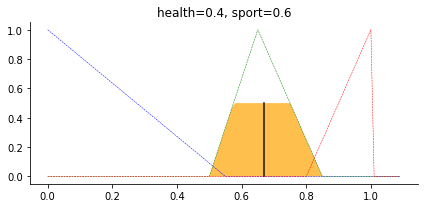
\includegraphics[width=\textwidth]{./pic/实验1.png} \\
        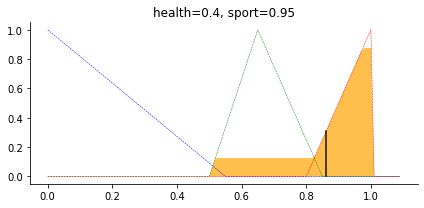
\includegraphics[width=\textwidth]{./pic/实验2.png}
    \end{tabular}
\caption{两组实验的模糊函数曲线}
\label{实验}
\end{figure}

\section{系统搭建与评估}

本研究搭建的系统分为前端和后端两部分。前端负责利用表单收集信息,后端负责计算带权加和得分以及推荐房源在地图的标注。

\subsection{前端}

系统前端为表单格式,用户填写希望寻找的房源类型、对不同区位需求的偏好程度、以及自身预算情况后,点击提交按钮即可将数据发送到服务器进行进一步的处理。其中,用户偏好被分为很同意、同意、无所谓、不同意、很不同意,对应的量化权值分别为2、1、0、-1、-2。服务器计算完毕后,页面将自动渲染地图,并在地图上标注出根据用户需求所推荐的房源信息。

\subsection{后端}

服务器由python的Django包搭建以支持相关网络工作。由于需要支持用户对于房源类型的需求以及考虑预算情况,后端仅能考虑满足这些条件的房源。通过预先定义好对应的类别字典,直接将前端传送的值从字典中查找出所对应的项,即可快速筛选出对应房源。

\begin{python}
HOME, HOTEL, BUSINESS = 0, 1, 2
ADEQUATE, NORMAL, SHORT = 0, 1, 2
estate_types_dict = {
    HOME: {
        ADEQUATE: ["住宅区", "商住两用楼宇", "别墅"],
        NORMAL: ["住宅区", "商住两用楼宇"],
        SHORT: ["住宅区"],
    },
    HOTEL: {
        ADEQUATE: ["宾馆酒店", "旅馆招待所", "经济型连锁酒店", "三星级宾馆", "四星级宾馆", "五星级宾馆", "青年旅舍"],
        NORMAL: ["宾馆酒店", "旅馆招待所", "经济型连锁酒店", "青年旅舍"],
        SHORT: ["旅馆招待所", "经济型连锁酒店", "青年旅舍"]
    },
    BUSINESS: {
        ADEQUATE: ["写字楼", "商住两用楼宇", "产业园区"],
        NORMAL: ["写字楼", "商住两用楼宇"],
        SHORT: ["商住两用楼宇"],
    },
}
\end{python}

通过上述类别对房源进行第一步筛选以后,需要利用用户选择的五项需求的权重向量计算每个房源的得分情况。每处房源五项区位需求的得分在数据处理阶段已经通过模糊推理预先计算完毕。因此,这里只需要将得分矩阵与权重向量做乘法,即可得到所有房源得分。对所有房源得分进行排序后,选出得分最高的几项作为推荐房源,并利用folium包在地图上进行标注。

\begin{python}
estates = pd.read_csv("../fuzzy_estates.csv")
def recommend(estate_type, weight, budget):
    types = estate_types_dict[estate_type][budget] #查找estate_type和budget对应类别
    estates = estates[estates["中类"].isin(types)] #根据类别筛选出房源
    estates.index = range(len(estates)) #重置行索引
    weight = np.array(weight)
    scores = estates.iloc[:, 9:].values #所有房源的五项得分
    scores = scores.dot(weight.T) #点乘权重向量
    index = (-scores).argsort() #获取降序排序的索引
    estates = estates.loc[index, :] #根据索引重新排序房源
    draw_map(estates.iloc[:5, :]) #在地图上标注出前五个房源
\end{python}

\subsection{系统评估}

实验显示,在不同场景下的两组提交均生成了满足用户需求的结果(图\ref{实际实验})。

当用户需要的房源类型为宾馆酒店且预算充足时,若其偏好于\textbf{消费}、\textbf{旅游}和\textbf{交通},则推荐的房源围绕在五角场附近。五角场内消费场所众多,并且附近有两座地铁站以及大量公交站台,同时东南方向还有两处风景优美的大型公园,无疑该处的房源很好地对应了用户选定的区位要求。

当用户需要的房源类型为家用住宅且预算一般时,若其仅仅偏好于\textbf{教育},则推荐的房源在中原路国和路附近。这里有大量的中小学以及幼儿园,还有一处文化园。对于用户教育资源需求来说,该处房源能够很好地满足。同时,所推荐地房源均为普通居民小区,也对应了用户预算一般的限制。

\begin{figure}[htbp]
\centering
    \begin{tabular}{c}
        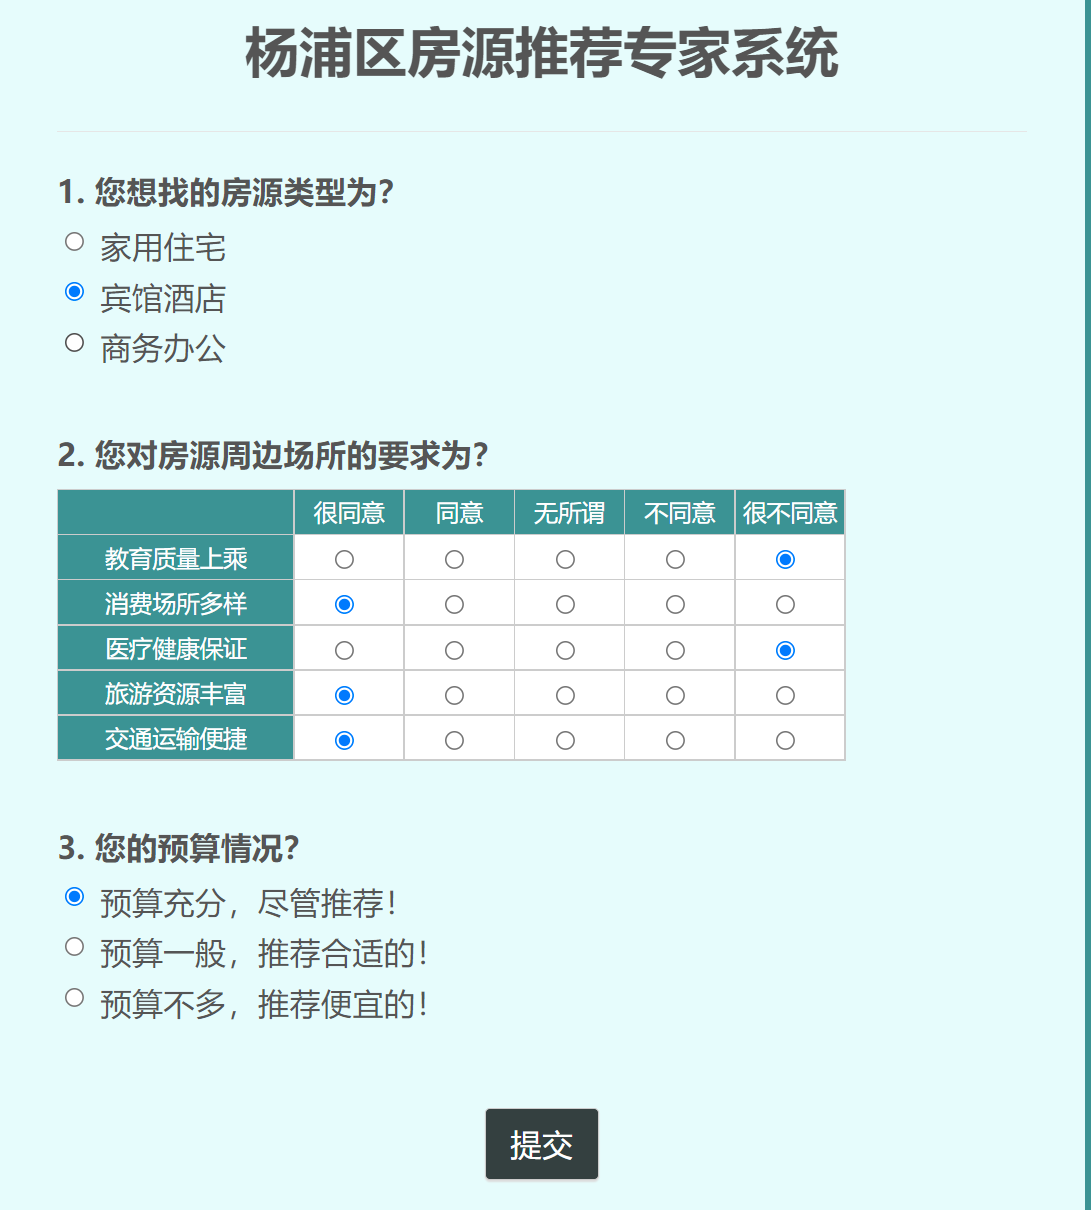
\includegraphics[width=0.5\textwidth]{./pic/用例1表单.png}
        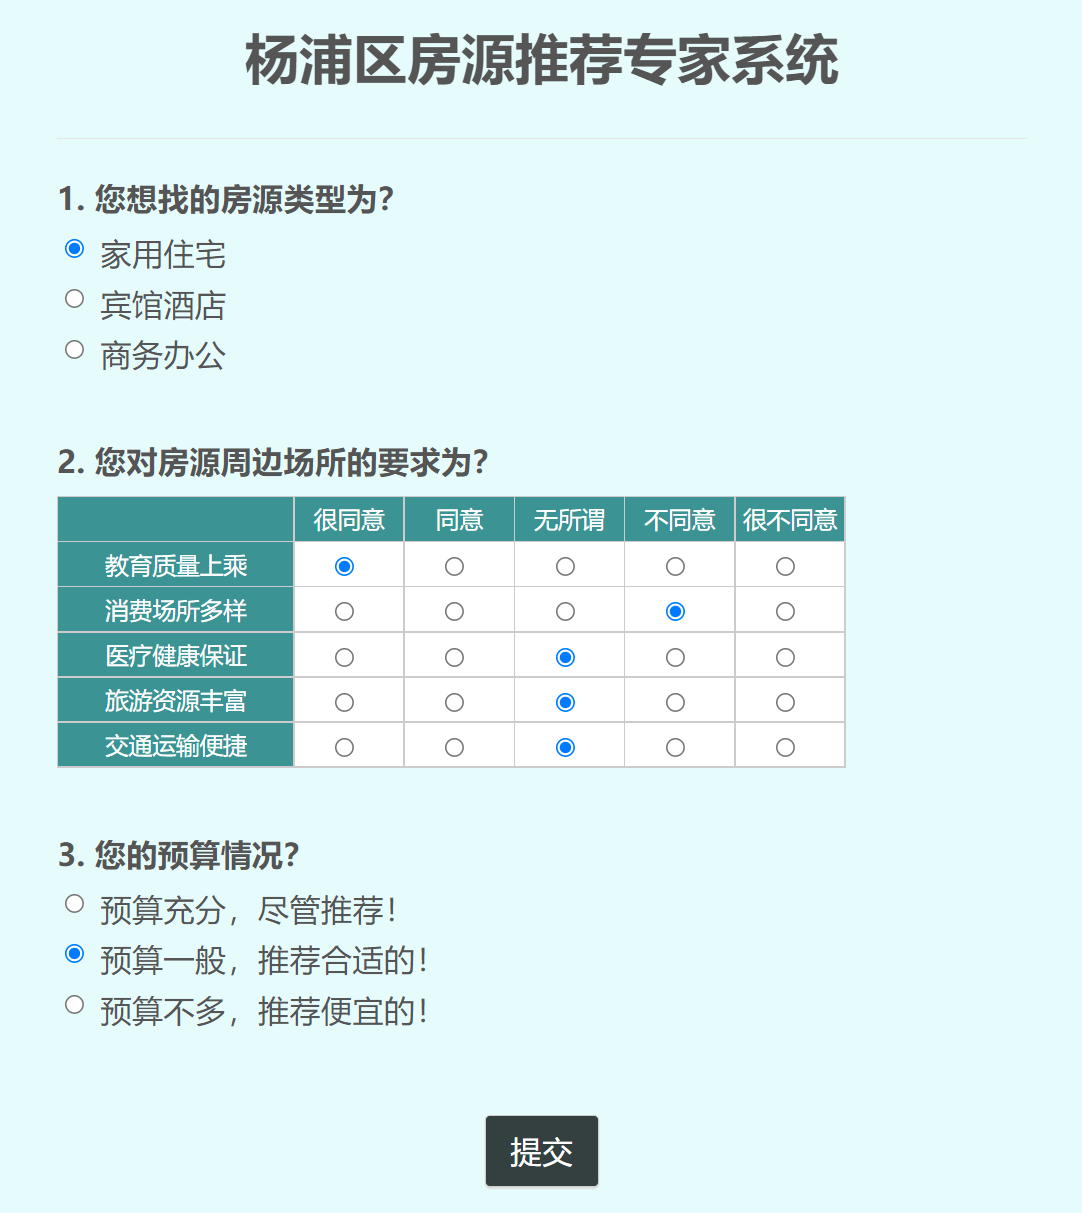
\includegraphics[width=0.5\textwidth]{./pic/用例2表单.png} \\
        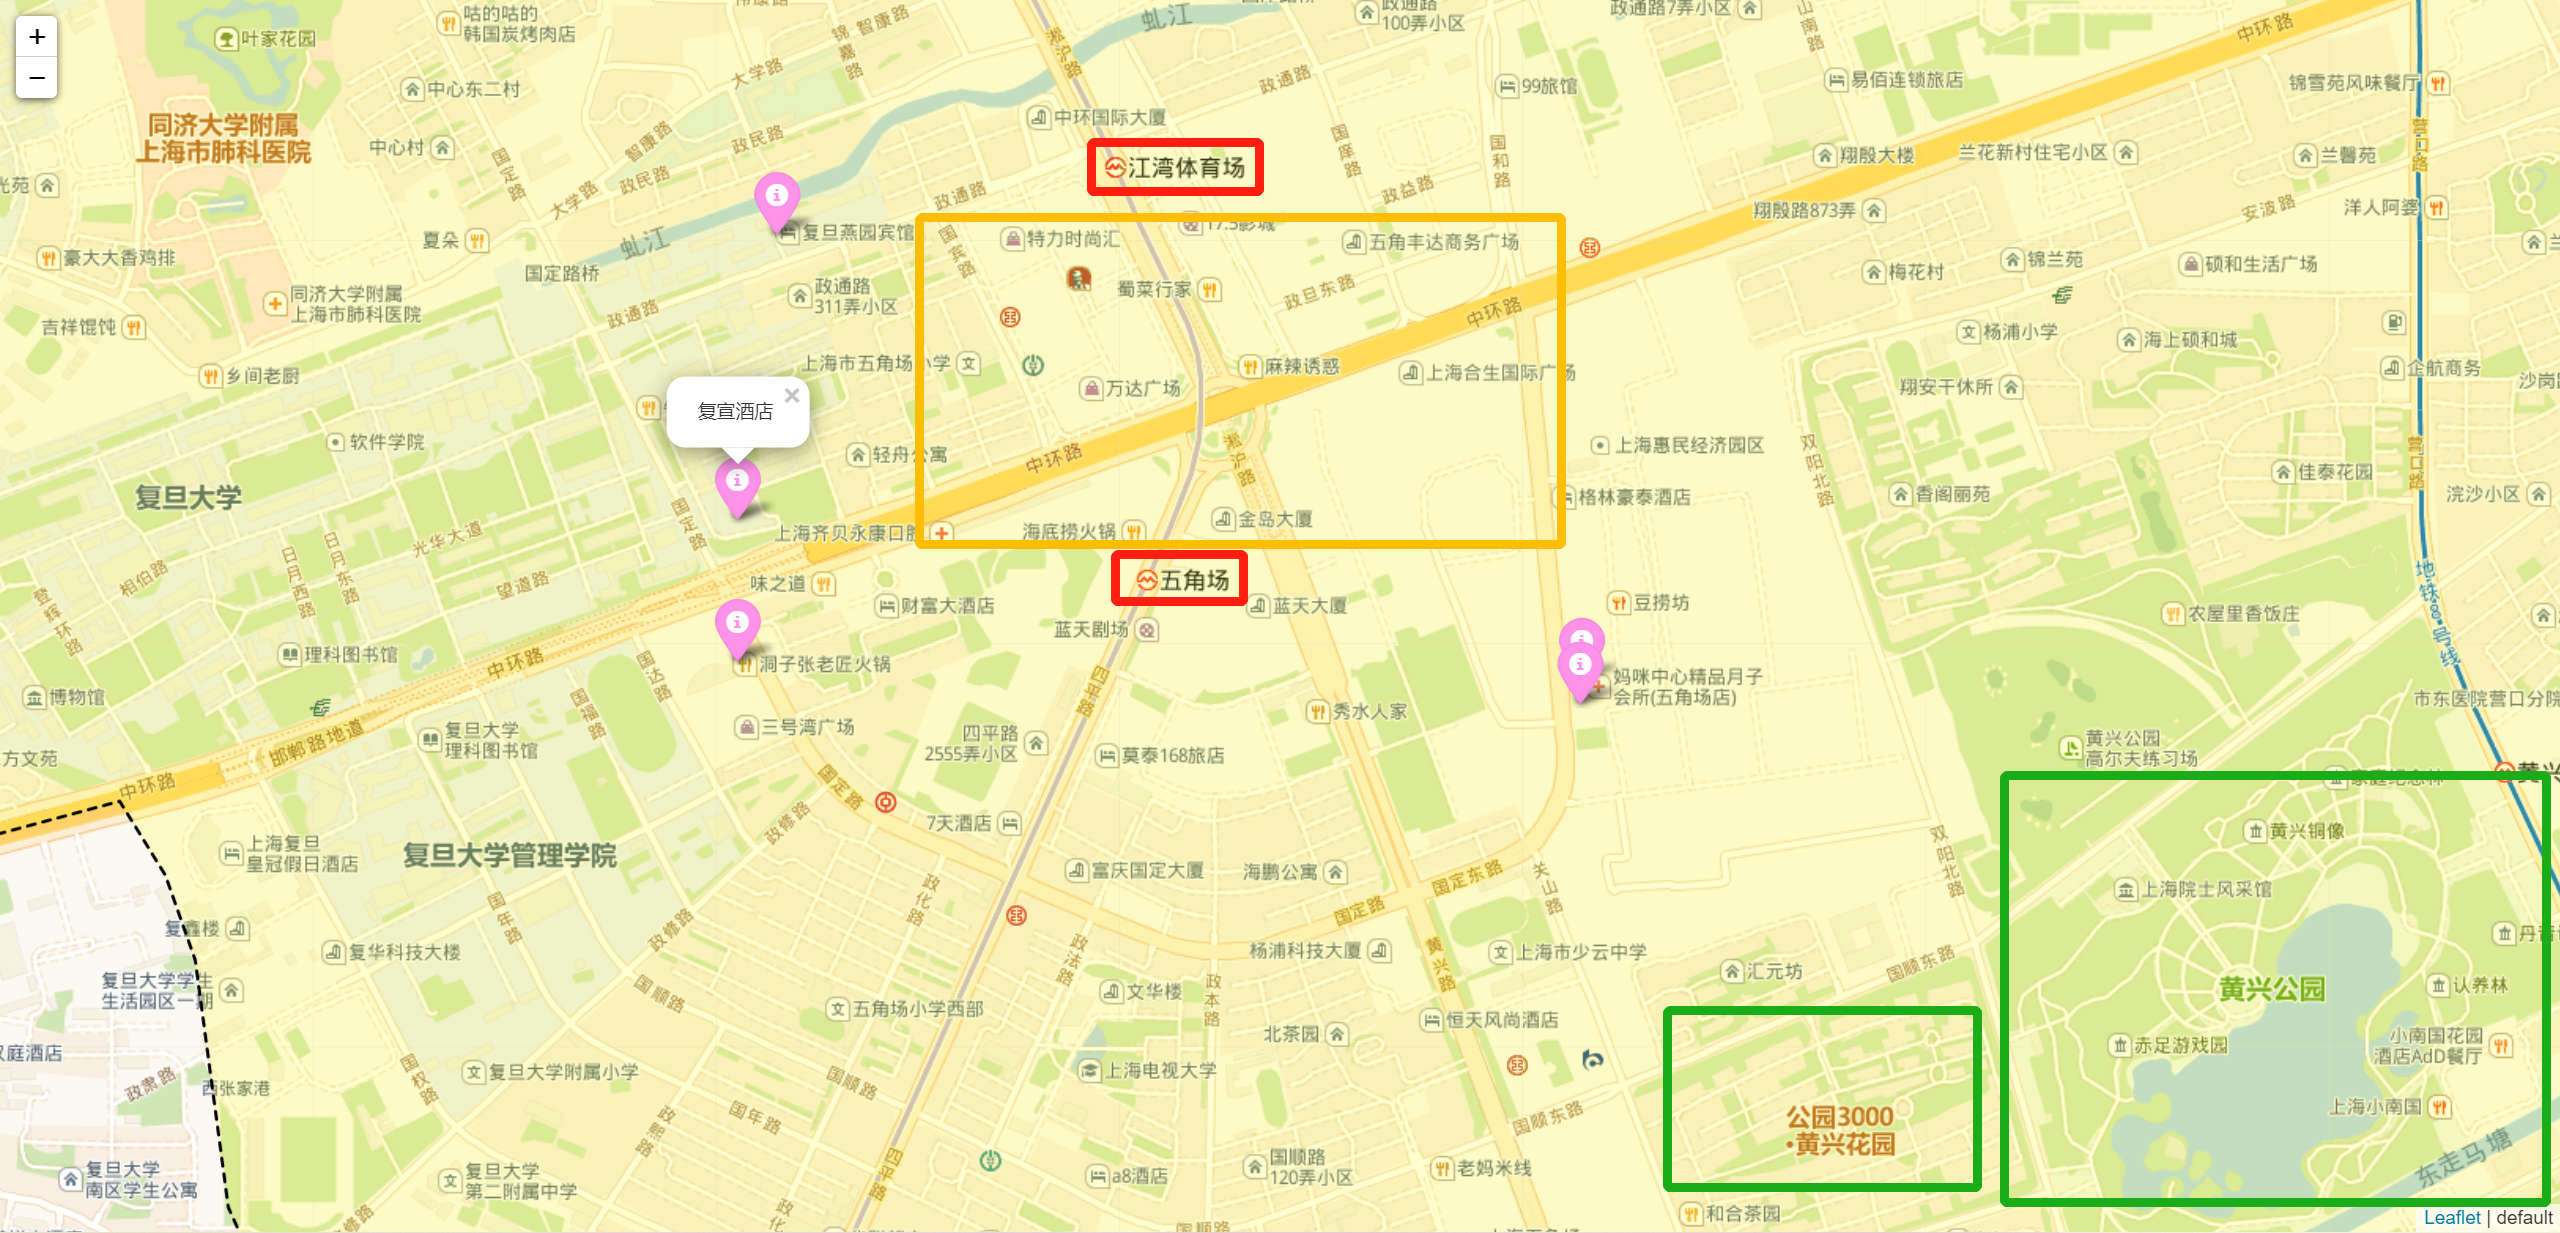
\includegraphics[width=\textwidth]{./pic/用例1结果.png} \\
        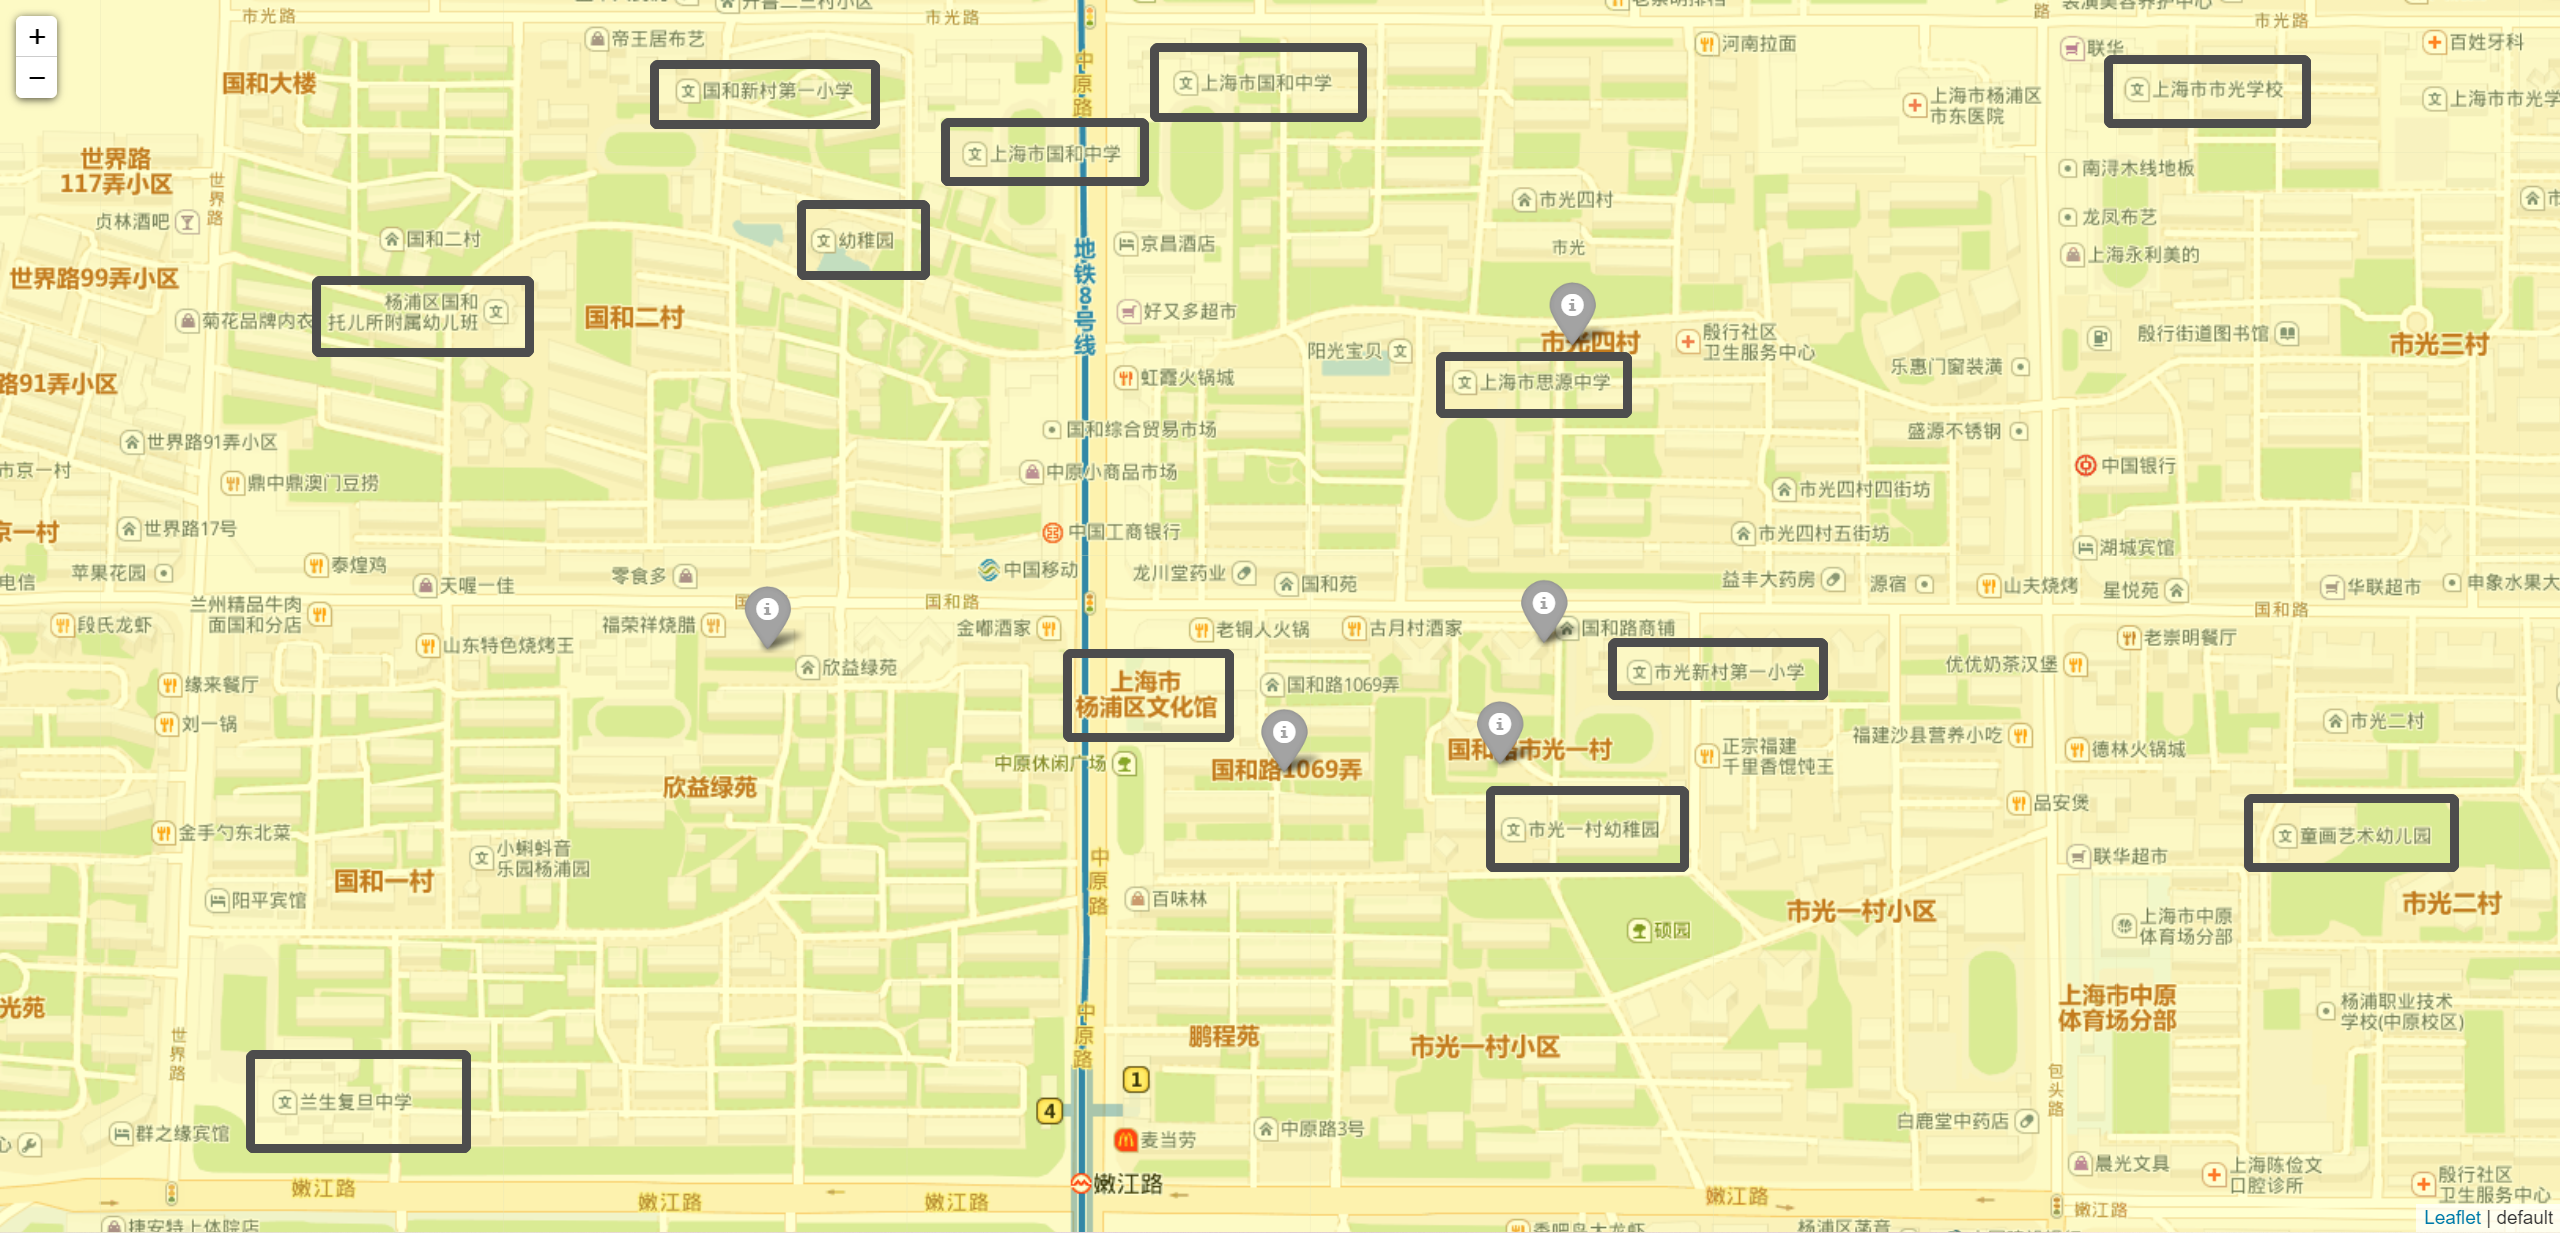
\includegraphics[width=\textwidth]{./pic/用例2结果.png}
    \end{tabular}
\caption{两组提交下系统的推荐结果}
\label{实际实验}
\end{figure}

\section{总结与展望}

本研究在模型的建构上还有改进的空间。例如在计算大类得分时,对于不同性质子类的设施给予不同权重的计分相对权重一致来说更为科学。然而本研究并未找到解决数据本身粗糙性的方法,因此未能实现该功能。在最终的房源推荐上,也可以加入筛选由用户指定位置周边房源的功能以更大程度提高用户自由度,由于地图直接拾取坐标的实现难度,该功能也暂未实现。这两点是本研究可以继续改进的地方。

总体来看,本研究构建了一个基于模糊推理的房源推荐系统,实现了对房源区位条件的综合分析,一定程度上满足了用户个性化需求,具有较好的应用价值。同时,在处理数据和构建系统过程中,本文作者也对模糊推理以及专家系统的相关知识有了更加深入的理解和掌握。

\begin{thebibliography}{6}

\bibitem{bg} 胡奕斐. 购房消费行为分析[J]. 杭州: 浙江工业大学, 2001.

\bibitem{需求分析} 孙聪, 刘霞, 姚玲珍. 新时代住房供应如何契合租购群体的差异化需求?[J]. 财经研究, 2019, 45(1): 75-88.

\bibitem{poi分类} Yin Z, Wu Y, Jin Z, et al. Research on livable community evaluation based on GIS[C]//IOP conference series: Earth and environmental science. IOP Publishing, 2018, 108(4): 042075.

\bibitem{walk} Score W. Walk score methodology[J]. Accessed April, 2014, 24.

\bibitem{folium} Journois M, Story R, Gardiner J, et al. python-visualization/folium v0. 12.1[J]. Zenodo.

\bibitem{skfuzzy} Warner J, Sexauer J, Unnikrishnan A. JDWarner/scikit-fuzzy: Scikit-Fuzzy version 0.4. 2[J]. Zenodo, 2019.

\end{thebibliography}

\end{document}
